\documentclass[11pt]{article}
\usepackage[T1]{fontenc}
\usepackage{listings}
\usepackage{xcolor}
\usepackage{graphicx}
\lstset { %
    language=C++,
    backgroundcolor=\color{black!5}, % set backgroundcolor
    basicstyle=\footnotesize,% basic font setting
}
\author{Piotr Popis}
\title{ Algorytmy realizowane przez system}
\date{29 maj}

\begin{document}
\begin{titlepage}
\maketitle 
\end{titlepage}
\section{Algorytm komponentów}
\subsection{Color Sensor}
\subsubsection{Słownie}
Kolor sensor przetwarza następujące procedury.
\begin{enumerate}

\item Wykrywa kolor obiektu, \item następnie wysyła sygnał do mikrokontrolera ,aby wykonać akcję.\item  Jest zintegrowany z 4 LED,które frontowo naświetlają obiekt. Wykrywają tak kolor w tablicy 64- fotodiod. Każdy czerwony, niebieski, zielony lub bez filtra. \item Określony zostaje kolor na podstawie natężenia odbicia światła. \item Mikrokontroler odbiera syngał z TCS.
\end{enumerate}
\subsection{Motor Servo}
\subsubsection{Słownie}
Jest to DC silnik, który kontroluje pozycję w krokach. Jest kontrolowany przez technikę modulacji pulsowej szerokości. Sygnał PWM ma długość około 20 ms. Szerokość pulsu ma od 1 do 2 ms. Długość pulsu determinuje jak daleko poruszy się silnik.
\subsubsection{Graficznie}
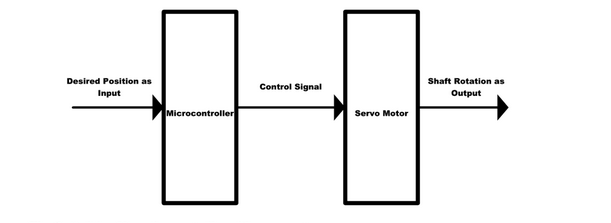
\includegraphics[scale=0.6]{serv.png}

\section{Algorytm w stanie aktywności}
\subsection{Słownie}
\begin{enumerate}
\item Wczytujemy kolor obiektu podanego przez serwo
\item Określamy czy udało się zbadać kolor ( wynik jest w zasięgu sensora), jeśli tak to szukamy odpowiedniego koloru, jeśli nie raise error
\item Doprowadzamy iteracyjnie nasze natężenia, czy ich kombinacja pasuje do któregoś koloru. Jeśli Tak przechodzimy do parsowania erroru, jeśli nie to sprawdzamy kolejne kolory aż do ostatniego - jeśli nie został zaimplementowany to "abstrakcyjnie raise error". 
\item Teraz jeśli mamy podniesiony sygnał erroru zsuw zostaje ustawiony pod kątem kontenera "error container", jeśli wykryto któryś z kolorów ustawiamy zsuw pod odpowiednim kątem do odpowiadającego zbiornika
\end{enumerate}
Czyli nasza obsługa błędów nie zmienia nic w działaniu po prostu obiekt jest zepchnięty do przeznaczonego do tego kontenera, powala to na uniknięcie " blokowania się obiektu podczas analizy, wewnątrz systemu".
\subsection{Diagram}
Rysunek przedstawia przybliżenie opisu słownego z punktu powyższego.\\
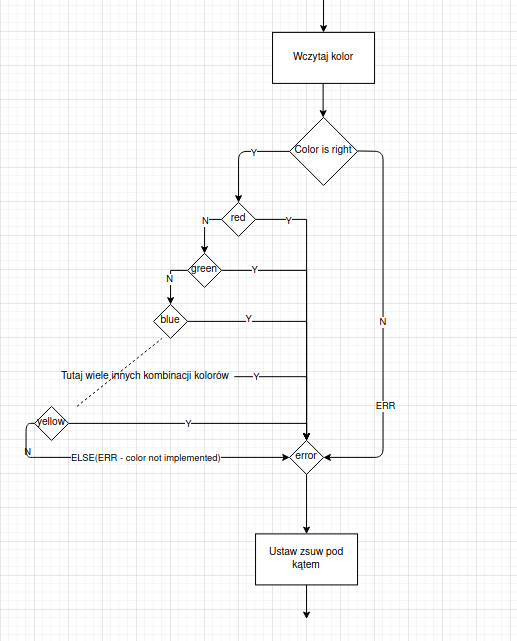
\includegraphics[scale=0.6]{act.png}
\section{Algorytm całego systemu w pseudokodzie}
\subsection{Pseudokod}
\begin{lstlisting}
loop(){
	moveSerwo1Degrees(X)
	color = detectColor()
	decision = chooseContainer(color)
	moveSerwo2(decision)
	pushObject()
	moveSerwo1Degrees(-X)
}

detectColor(){
//sprawdzamy czerwone
	digitalWrite(X, LOW);
	digitalWrite(X, LOW);
	R = pulseIn(sensor,LOW);
//sprawdzamy zielone
	digitalWrite(X, LOW);
	digitalWrite(X, HIGH);
	G = pulseIn(sensor,LOW);
//sprawdzamy niebieskie
	digitalWrite(X, HIGH);
	digitalWrite(X, HIGH);
	B = pulseIn(sensor,LOW);
	color = colorCombinations(R,G,B);
	return color;
}

colorCombinations(R,G,B){
	if(R> 24 and R < 38 and G> 30 and G<44)\{
		color = 1 // yellow 
	}
	if(B> 22 and B < 19 and G> 22 and G<25)\{
		color = 2 // orange 
	}
	.
	.
	.
	return  color;
}

chooseContainer(color){
	if(color == 1){
		serwo.write(X);
	}
	if(color == 2){
		serwo.write(X);
	}
	.
	.
	.
}
\end{lstlisting}
\end{document}